 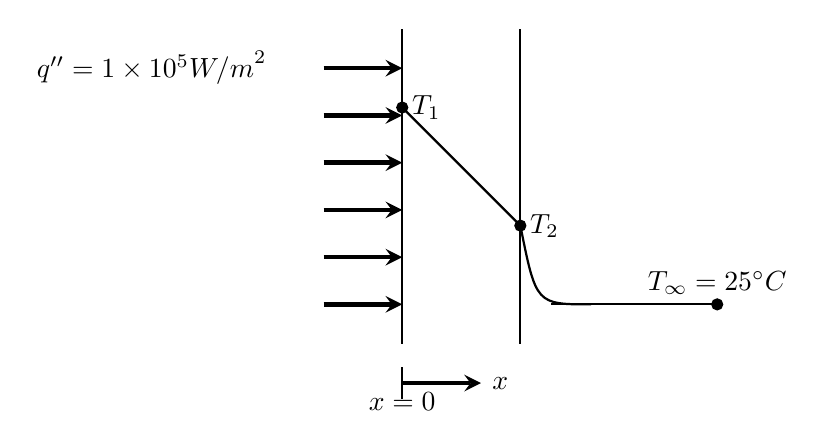
\begin{tikzpicture}
   
    \draw[thick] (0,-2) -- (0,2);
\draw[thick] (1.5,-2) -- (1.5,2);
  
    \foreach \y in {-1.5, -0.9, -0.3, 0.3, 0.9, 1.5} {
        \draw[->, ultra thick,>=stealth] (-1, \y) -- (0, \y);
    }

   
    \node[left] at (-1.6, 1.5) {$q'' = 1 \times 10^5  \text{ W/m}^2$};

    
    \filldraw (0, 1) circle (2pt) node[right] {$T_1$};
    \filldraw (1.5, -0.5) circle (2pt) node[right] {$T_2$};
    \filldraw (4, -1.5) circle (2pt) node[above] {$T_\infty = 25^\circ\text{C}$};

   
    \draw[thick] (0,1) -- (1.5,-0.5); 
    \draw[thick] (1.5,-0.5) .. controls(1.7,-1.5)..(2.4,-1.5); 
\draw[thick] (4,-1.5)--(1.89,-1.5);
   
   \draw[->, ultra thick, >=stealth] (0, -2.5) -- (1, -2.5) node[right] {$x$};
    
  
    \draw[thick] (0, -2.3) -- (0, -2.7);
    
   
    \node[below] at (0, -2.5) {$x=0$};
\end{tikzpicture}
